
\chapter{Introduction}


Most scholars focus on power as a means, the strength or capacity that provides the “ability to influence the behavior of other actors in accordance with one’s own objectives.” – David Jablonsky

Power is the ability to achieve one’s purposes or goals – Joseph Nye

Power is the ability to get others to do what they otherwise would not do – Robert Dahl


\epigraph{“But neither can the weak states ever afford to relax their vigilance on matters of security, nor bask in the protection and good will of the powers.”}{\parencite{HANDEL_2005}}

\section*{Introduction}
This chapter shall introduce the debate regarding the influence of small states on security outcomes. It provides a conceptual understanding of a small state, explains why it is assessed that `conditional legitimacy' emerges as the centre of gravity. While considering legitimacy, the essay explore how national history and myths shape national identity and legitimacy. It consider possible `problem states' whose influence appears malleable based on the lens applied. The author suggests a five-effects framework, upon which the question is analysed. These are, niche specialisation, organisational agility, hybrid leverage, soft-power synergy and conditional legitimacy. 


\section*{Defining Small States}
No consensus emerges from the literature regarding definition or approach to state `size'. As noted by BECKLEY (2018) \nocite{BECKLEY_2018,CROWARDS_2002}, a simple numerical method is often applied comprising: GDP; population; landmass; military spending. These metrics focus on power. While power and influence aren't synonymous, realists contend that power brings influence\footnote{While believing that the converse isn't true}. On this basis, states such as Ireland  and Qatar are small since they cannot affect the balance of power unilaterally. A more reflexive approach was taken by \textcite{KEOHANE_1969}, where the a neorealist `systemic role' is considered.  Influential small states may therefore be described to be ``system affecting'' due their position within the international order. A more nuanced approach, grounded in concepts of influence was considered by \textcite{THORHALLSSON_2006}. It included concepts of sovereignty size, political size (domestic cohesion), perceptual size (international opinions) and preference size (ambitions). Thorhallsson's concepts of `action capacity' and vulnerability refines the Keohane's systemic role of small states, while his considerations within the state are realist in nature. Liberal institutionalism facilitates small states to maximise influence in peacetime through multilateral cooperation\parencite{FARRELL_2019}. Mearsheimer's (1994) cautions of the influence of international institutions. This is echoed by \textcite{BESSNER_2015}, who critique that by disregarding national considerations, neorealism strips out national decision makers. It lots states into a anarchic system and structural adaptation. These perspectives sharpen the hypothesis that small states have a limited unilateral capacity for action. They must adapt to the structures and great powers around them. Given overlapping definitions and an absence of consensus, this essay prioritises a neorealist systematic perspective. It is grounded in capacity, vulnerability and institutional positioning.

\section*{Legitimacy as the Centre of Gravity}
Legitimacy emerges as the true COG for small states. With limited military capacity, this aspect of influence is marginalised. It can neither decisively affect change nor alter the balance of power through token gestures. Nevertheless, legitimacy allows small states to justify their actions within norms and institutions. Ireland's UN participation illustrates this dynamic. While materially limited, she appears to have gained disproportionate international recognition by presenting the Defence Forces as impartial and committed to collective security \parencite{ROTHSTEIN_1968}.

Legitimacy acts within and without the state. It sustains domestic support for engagement overseas. It amplifies small states' voices within institutions. 



 


Also in 1969, Waltz's seminal structural-realist book \textit{Theory of International Politics} was published. Although neorealists are distrustful of institutions, small states may be afforded the opportunity to influence the system through them.


Soft power is that which is not coercive. To many (perhaps most), soft power is a weaker capability than hard power (which is coercive). It seems that the most powerful is in fact the use of soft power when you already have hard power. Said differently, having hard power and not using it is the highest form of power. I suggest that there is an analogue here with leadership. Command is a legal authority bestowed on an individual. However, authority is given to a person by their subordinates, where they get what they want through influence rather than coercion. 

So, for small states whose only meaningful tools are soft power, then they are bounded because their use of soft power isn't necessarily virtuous. They're not employing hard power because they choose not to, in favour of soft power. They're not employing hard power because they don't have it to begin with. Covnersely, a large power is virtuous by not using hard power.


Gray's 2005 \nocite{GRAY_2005}'s critique of U.S. post-Cold-War failure highlights another form of small state influence - through chaos. Indeed, unscrupulous leaders could weaponise what a functioning state would consider as a vulnerability. This was warned of by Hirst (2010) \nocite{HIRST_2010} regarding Lebanon. The key to such perverse success is the great power's political home front. Such small states could be resistant to coercive diplomacy, perhaps as DPRK today.

Mearshimer's 1994 \nocite{MEARSHIMER_1994} and Keohane \nocite{KEOHANE_1969} disagree. Keohane is a liberal institutionalisation, while Mearshimer critique is much more compelling. The core weakness of instutionalism is that of cheating and relative gains. While instutionalism for economic relations appears logical, the two-steps-forward one-step-back feature of cooperation are incompatible with security concerns. Hence realists' skepticism towards liberalism. For small states, in a purely realist world, their influence is minimised. During peacetime however, liberal institutionalism can be leveraged to achieve influence. 


\textcite{HINTON_2020} notes that the stability brought about by international cooperation following the second word war was not as stable as claimed. This echoes \textcite{MEARSHEIMER_1994} conclusion that while it has been popular to praise institutionalism and the `liberal rules-based order', evidence attributing it to success at avoiding war is doubtful.

The following figures illustrate a thought-experiment, based upon the author's perceptions. They are intended ot motivate the concept that small states' influence cannot be meaningfully represented by the traditional metrics. On material metrics, Ireland's influence is comparable to dysfunctional states. 
\begin{table}[ht]
	\centering
	\begin{tabular}{p{2.8cm} p{1.5cm} p{1.8cm} p{2cm} p{1.8cm} p{2cm}}
		\hline
		\textbf{State} & \textbf{Size (0–10)} & \textbf{Capacity (0–10)} & \textbf{Perception (0–10)} & \textbf{Total (/60)} & \textbf{Category} \\
		\hline
		South Sudan & 4 & 2 & 3 & 17 & Fragile Small \\
		Somalia & 3 & 2 & 4 & 19 & Fragile Small \\
		Lebanon & 3 & 3 & 4 & 22 & Fragile Small \\
		Sudan & 7 & 3 & 4 & 24 & Fragile Small \\
		Syria & 6 & 4 & 5 & 25 & Fragile Small \\
		Iraq & 6 & 4 & 5 & 25 & Fragile Small \\
		Qatar & 2 & 9 & 8 & 28 & Microstate \\
		Ireland & 4 & 7 & 8 & 29 & Functional Small \\
		Singapore & 2 & 10 & 9 & 29 & Microstate \\
		Denmark & 4 & 8 & 8 & 30 & Functional Small \\
		North Korea & 5 & 7 & 5 & 31 & Exceptional Small \\
		Israel & 4 & 9 & 5 & 32 & Exceptional Small \\
		Finland & 5 & 9 & 9 & 32 & Functional Small \\
		South Africa & 7 & 7 & 7 & 36 & Middle Power \\
		Nigeria & 9 & 6 & 6 & 36 & Middle Power \\
		Iran & 9 & 8 & 8 & 40 & Middle Power \\
		Russia & 10 & 8 & 9 & 45 & Great Power \\
		Japan & 8 & 10 & 10 & 48 & Great Power \\
		UK & 10 & 10 & 10 & 50 & Great Power \\
		Germany & 10 & 10 & 10 & 50 & Great Power \\
		France & 10 & 10 & 10 & 50 & Great Power \\
		USA & 10 & 10 & 10 & 60 & Superpower \\
		China & 10 & 10 & 10 & 60 & Superpower \\
		\hline
	\end{tabular}
	\caption{Thorhallsson’s qualitative criteria applied to selected states. Scores reflect size, capacity, perception; categories highlight relative status.}
\end{table}

\begin{table}[ht]
	\centering
	\begin{tabular}{p{2.8cm} p{1.8cm} p{1.8cm} p{1.8cm} p{1.8cm} p{1.8cm}}
		\hline
		\textbf{State} & \textbf{Landmass} & \textbf{Population} & \textbf{Military} & \textbf{GDP} & \textbf{Total (/40)} \\
		\hline
		Lebanon & 2 & 3 & 2 & 3 & 10 \\
		South Sudan & 6 & 3 & 2 & 2 & 13 \\
		Somalia & 6 & 4 & 2 & 2 & 14 \\
		Syria & 5 & 5 & 2 & 3 & 15 \\
		Qatar & 1 & 2 & 5 & 10 & 18 \\
		Ireland & 3 & 3 & 4 & 8 & 18 \\
		Iraq & 6 & 6 & 3 & 5 & 20 \\
		Sudan & 8 & 6 & 3 & 3 & 20 \\
		Singapore & 1 & 2 & 7 & 10 & 20 \\
		Denmark & 4 & 3 & 5 & 10 & 22 \\
		North Korea & 5 & 6 & 8 & 3 & 22 \\
		Finland & 7 & 4 & 7 & 8 & 26 \\
		Israel & 3 & 3 & 9 & 9 & 28 \\
		South Africa & 8 & 7 & 5 & 8 & 28 \\
		Nigeria & 9 & 9 & 6 & 5 & 29 \\
		Iran & 9 & 8 & 7 & 6 & 30 \\
		Russia & 10 & 9 & 9 & 8 & 36 \\
		Germany & 6 & 8 & 6 & 10 & 36 \\
		Japan & 5 & 9 & 6 & 10 & 36 \\
		France & 7 & 7 & 9 & 10 & 37 \\
		UK & 6 & 8 & 9 & 10 & 37 \\
		China & 10 & 10 & 10 & 10 & 40 \\
		USA & 10 & 10 & 10 & 10 & 40 \\
		\hline
	\end{tabular}
	\caption{Traditional material criteria (landmass, population, military, GDP) applied to selected states.}
\end{table}

\pgfplotsset{compat=1.18}

\pgfplotsset{compat=1.18}

% Normalised Thorhallsson Chart
\begin{figure}[ht]
	\centering
	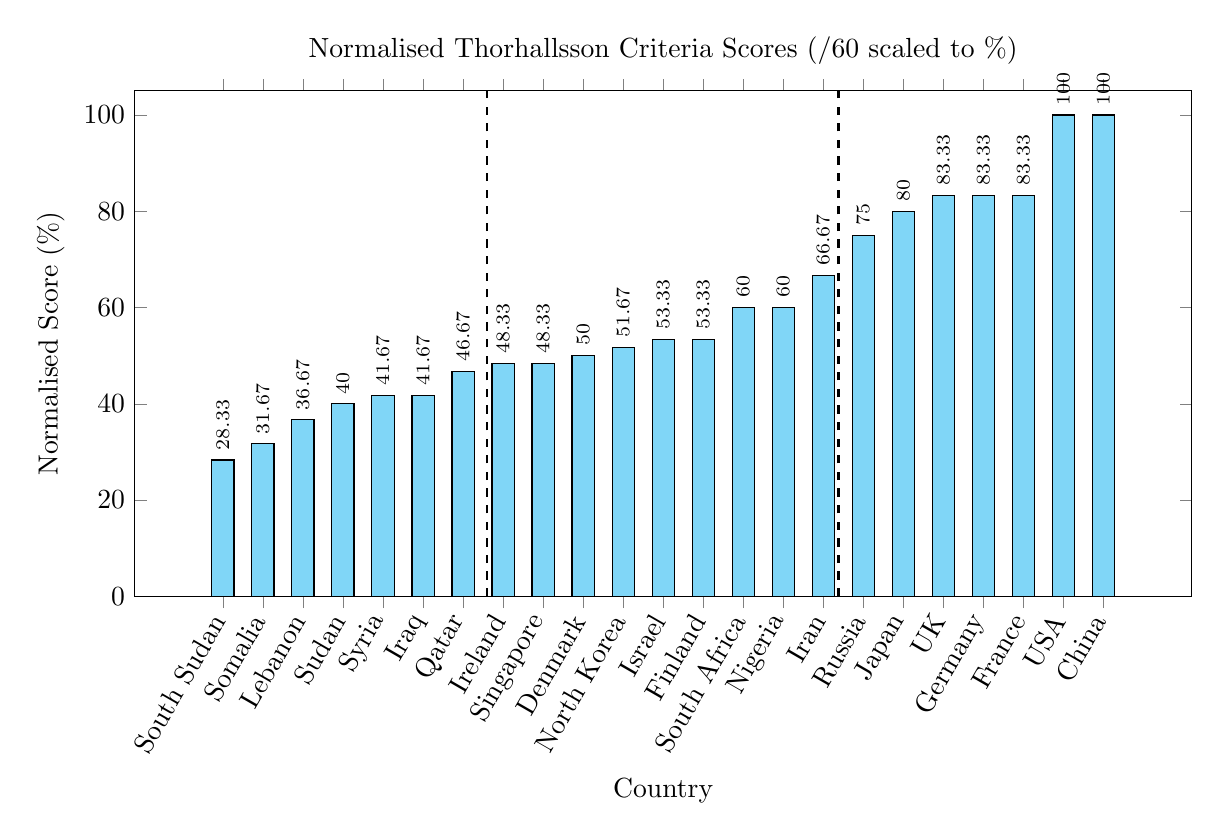
\begin{tikzpicture}
		\begin{axis}[
			ybar,
			bar width=8pt,
			width=15cm,
			height=8cm,
			ylabel={Normalised Score (\%)},
			xlabel={Country},
			symbolic x coords={SouthSudan,Somalia,Lebanon,Sudan,Syria,Iraq,Qatar,Ireland,Singapore,Denmark,NorthKorea,Israel,Finland,SouthAfrica,Nigeria,Iran,Russia,Japan,UK,Germany,France,USA,China},
			xtick=data,
			xticklabels={South Sudan,Somalia,Lebanon,Sudan,Syria,Iraq,Qatar,Ireland,Singapore,Denmark,North Korea,Israel,Finland,South Africa,Nigeria,Iran,Russia,Japan,UK,Germany,France,USA,China},
			x tick label style={rotate=60, anchor=east},
			ymin=0,ymax=105,
			nodes near coords,
			every node near coord/.append style={font=\scriptsize, rotate=90, anchor=west, text=black},
			nodes near coords align={center},
			title={Normalised Thorhallsson Criteria Scores (/60 scaled to \%)}
			]
			
			\addplot+[ybar, fill=cyan!50, draw=black, nodes near coords] coordinates {
				(SouthSudan,28.33) (Somalia,31.67) (Lebanon,36.67) (Sudan,40.00) (Syria,41.67) (Iraq,41.67)
				(Qatar,46.67) (Ireland,48.33) (Singapore,48.33) (Denmark,50.00) (NorthKorea,51.67) (Israel,53.33)
				(Finland,53.33) (SouthAfrica,60.00) (Nigeria,60.00) (Iran,66.67) (Russia,75.00) (Japan,80.00)
				(UK,83.33) (Germany,83.33) (France,83.33) (USA,100.00) (China,100.00)
			};
			
			% Vertical dashed lines at 1/3 and 2/3
			\draw[dashed, thick] (rel axis cs:0.333,0) -- (rel axis cs:0.333,1);
			\draw[dashed, thick] (rel axis cs:0.666,0) -- (rel axis cs:0.666,1);
			
		\end{axis}
	\end{tikzpicture}
	\caption{Normalised Thorhallsson scores (scaled to percentages).}
\end{figure}


% Normalised Traditional Chart
\begin{figure}[ht]
	\centering
	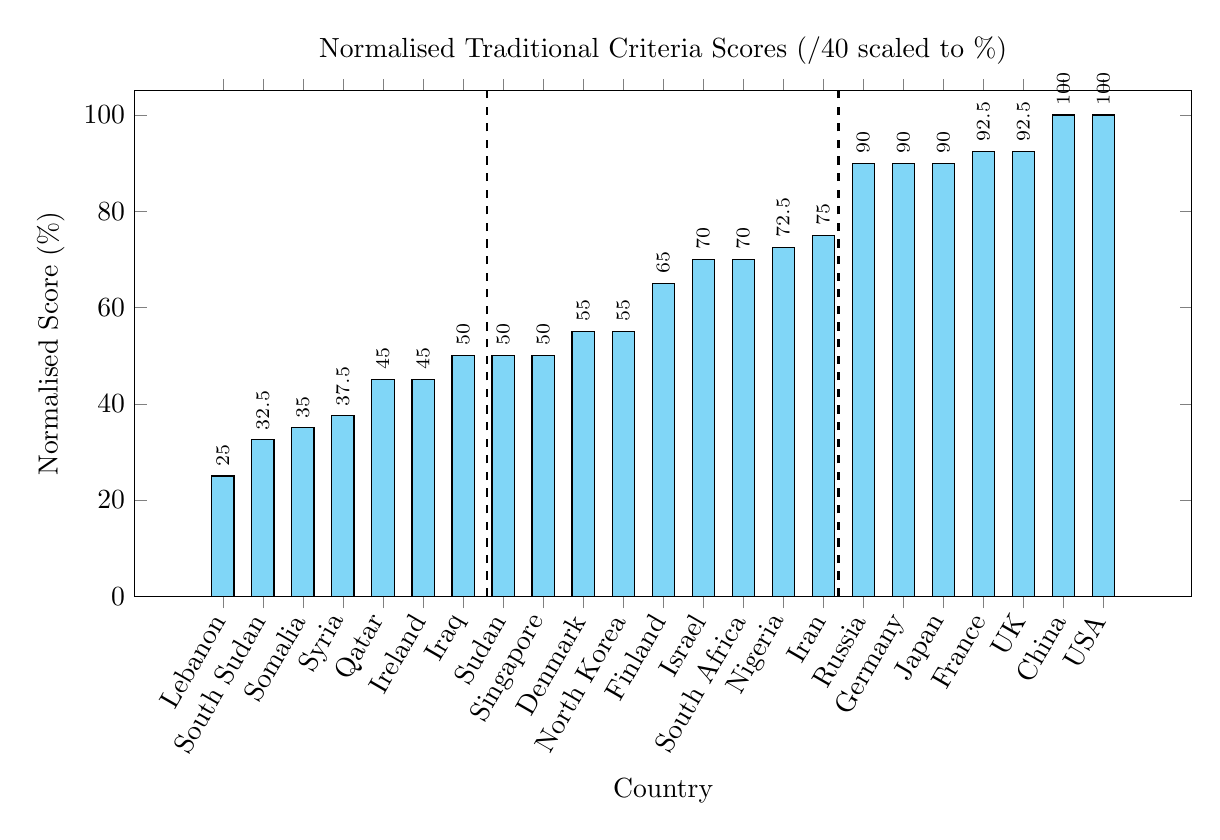
\begin{tikzpicture}
		\begin{axis}[
			ybar,
			bar width=8pt,
			width=15cm,
			height=8cm,
			ylabel={Normalised Score (\%)},
			xlabel={Country},
			symbolic x coords={Lebanon,SouthSudan,Somalia,Syria,Qatar,Ireland,Iraq,Sudan,Singapore,Denmark,NorthKorea,Finland,Israel,SouthAfrica,Nigeria,Iran,Russia,Germany,Japan,France,UK,China,USA},
			xtick=data,
			xticklabels={Lebanon,South Sudan,Somalia,Syria,Qatar,Ireland,Iraq,Sudan,Singapore,Denmark,North Korea,Finland,Israel,South Africa,Nigeria,Iran,Russia,Germany,Japan,France,UK,China,USA},
			x tick label style={rotate=60, anchor=east},
			ymin=0,ymax=105,
			nodes near coords,
			every node near coord/.append style={font=\scriptsize, rotate=90, anchor=west, text=black},
			nodes near coords align={center},
			title={Normalised Traditional Criteria Scores (/40 scaled to \%)}
			]
			
			\addplot+[ybar, fill=cyan!50, draw=black, nodes near coords] coordinates {
				(Lebanon,25.00) (SouthSudan,32.50) (Somalia,35.00) (Syria,37.50)
				(Qatar,45.00) (Ireland,45.00) (Iraq,50.00) (Sudan,50.00) (Singapore,50.00)
				(Denmark,55.00) (NorthKorea,55.00) (Finland,65.00) (Israel,70.00)
				(SouthAfrica,70.00) (Nigeria,72.50) (Iran,75.00) (Russia,90.00) (Germany,90.00)
				(Japan,90.00) (France,92.50) (UK,92.50) (China,100.00) (USA,100.00)
			};
			
			% Vertical dashed lines at 1/3 and 2/3
			\draw[dashed, thick] (rel axis cs:0.333,0) -- (rel axis cs:0.333,1);
			\draw[dashed, thick] (rel axis cs:0.666,0) -- (rel axis cs:0.666,1);
			
		\end{axis}
	\end{tikzpicture}
	\caption{Normalised traditional material scores (scaled to percentages).}
\end{figure}
